\part{Vue NPM}



\section{Node}


\begin{lstlisting}[language=bash]
$ curl -sL https://deb.nodesource.com/setup_7.x | sudo -E bash -
$ sudo apt-get install -y nodejs
$ node -v
v7.5.0
$ nodejs -v
v7.5.0
$ npm -v
4.1.2
\end{lstlisting}


\section{NPM}

\begin{lstlisting}[language=bash]
$ npm install -g npm@latest
$ npm -v
4.1.2
\end{lstlisting}

进入/path/to/hitour/themes/kitchen安装项目依赖:


\begin{lstlisting}[language=bash]
$ cd /path/to/hitour/themes/kitchen
$ sudo npm i
\end{lstlisting}

\begin{figure}[htbp]
\centering
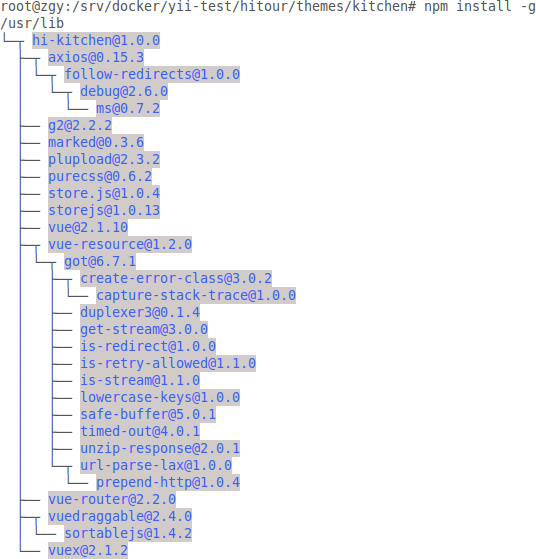
\includegraphics[scale=0.4]{kitchen-dependence.png}
\caption{kitchen项目前端依赖关系}
\end{figure}


创建本地的前端开发服务器配置文件/path/to/hitour/themes/kitchen/config/index.js,index.js的内容如下:

\begin{lstlisting}[language=JavaScript]
var path = require('path')

var common_proxy = {
  //target       : 'http://test.hitour.cc',
  //target       : 'http://sandbox.hitour.cc',
  target: 'http://trial.hitour.cc',
  // target       : 'http://hitour.host',
  changeOrigin: true,
  pathRewrite: {}
};

module.exports = {
  build: {
    env: require('./prod.env'),
    index: path.resolve(__dirname, '../dist/index.html'),
    assetsRoot: path.resolve(__dirname, '../dist'),
    assetsSubDirectory: 'static',
    assetsPublicPath: '/themes/kitchen/dist/',
    productionSourceMap: true,
    productionGzip: false,
    productionGzipExtensions: ['js', 'css']
  },
  dev: {
    env: require('./dev.env'),
    port: 60003,
    assetsSubDirectory: 'static',
    assetsPublicPath: '/',
    proxyTable: {
      '/admin/': common_proxy,
      '/chef/': common_proxy,
      '/themes': common_proxy,
      '/markMi/': common_proxy
    },
    cssSourceMap: false
  }
}
\end{lstlisting}

在/path/to/hitour/themes/kitchen目录下启动本地测试服务器,并且在\url{http://localhost:10003/k/sign\_in}进行测试。

\begin{lstlisting}[language=bash]
$ cd /path/to/hitour/themes/kitchen
$ npm run dev
\end{lstlisting}

如果本地测试通过,可以执行\texttt{npm run build}进行发布。

\begin{lstlisting}[language=bash]
$ cd /path/to/hitour/themes/kitchen
$ npm run build
\end{lstlisting}

注意,在本地或远程服务器做发布之前, 需要确认Yii的路由配置。

\subsection{access}

\begin{lstlisting}[language=bash]

\end{lstlisting}

\subsection{adduser}

\begin{lstlisting}[language=bash]

\end{lstlisting}

\subsection{bin}


\begin{lstlisting}[language=bash]

\end{lstlisting}

\subsection{bugs}


\begin{lstlisting}[language=bash]

\end{lstlisting}

\subsection{c}



\begin{lstlisting}[language=bash]

\end{lstlisting}

\subsection{cache}


\begin{lstlisting}[language=bash]

\end{lstlisting}

\subsection{completion}



\begin{lstlisting}[language=bash]

\end{lstlisting}

\subsection{config}


\begin{lstlisting}[language=bash]
$ npm config list

\end{lstlisting}

\subsection{ddp}


\begin{lstlisting}[language=bash]

\end{lstlisting}

\subsection{dedupe}



\begin{lstlisting}[language=bash]

\end{lstlisting}

\subsection{deprecate}




\begin{lstlisting}[language=bash]

\end{lstlisting}

\subsection{dist-tag}


\begin{lstlisting}[language=bash]

\end{lstlisting}

\subsection{docs}



\begin{lstlisting}[language=bash]
$ npm docs vue
\end{lstlisting}



\begin{lstlisting}[language=bash]
$ npm docs webpack
\end{lstlisting}


\begin{lstlisting}[language=bash]

\end{lstlisting}



\begin{lstlisting}[language=bash]

\end{lstlisting}

\subsection{doctor}



\begin{lstlisting}[language=bash]

\end{lstlisting}

\subsection{edit}



\begin{lstlisting}[language=bash]

\end{lstlisting}

\subsection{explore}



\begin{lstlisting}[language=bash]

\end{lstlisting}

\subsection{get}



\begin{lstlisting}[language=bash]

\end{lstlisting}

\subsection{help}



\begin{lstlisting}[language=bash]

\end{lstlisting}

\subsection{help-search}

\begin{lstlisting}[language=bash]

\end{lstlisting}

\subsection{i}


\begin{lstlisting}[language=bash]

\end{lstlisting}

\subsection{init}


\begin{lstlisting}[language=bash]

\end{lstlisting}

\subsection{install}


\begin{lstlisting}[language=bash]

\end{lstlisting}

\subsection{install-test}


\begin{lstlisting}[language=bash]

\end{lstlisting}

\subsection{it}


\begin{lstlisting}[language=bash]

\end{lstlisting}

\subsection{link}


\begin{lstlisting}[language=bash]

\end{lstlisting}

\subsection{list}


\begin{lstlisting}[language=bash]

\end{lstlisting}

\subsection{ln}



\begin{lstlisting}[language=bash]

\end{lstlisting}

\subsection{login}



\begin{lstlisting}[language=bash]

\end{lstlisting}

\subsection{logout}



\begin{lstlisting}[language=bash]

\end{lstlisting}

\subsection{ls}



\begin{lstlisting}[language=bash]

\end{lstlisting}

\subsection{outdated}


\begin{lstlisting}[language=bash]

\end{lstlisting}


\subsection{owner}


\begin{lstlisting}[language=bash]

\end{lstlisting}

\subsection{pack}


\begin{lstlisting}[language=bash]

\end{lstlisting}

\subsection{ping}



\begin{lstlisting}[language=bash]

\end{lstlisting}

\subsection{prefix}


\begin{lstlisting}[language=bash]

\end{lstlisting}

\subsection{prune}

\begin{lstlisting}[language=bash]

\end{lstlisting}

\subsection{publish}


\begin{lstlisting}[language=bash]

\end{lstlisting}

\subsection{rb}



\begin{lstlisting}[language=bash]

\end{lstlisting}

\subsection{rebuild}




\begin{lstlisting}[language=bash]

\end{lstlisting}

\subsection{repo}


\begin{lstlisting}[language=bash]

\end{lstlisting}

\subsection{restart}

\begin{lstlisting}[language=bash]

\end{lstlisting}

\subsection{root}


\begin{lstlisting}[language=bash]

\end{lstlisting}

\subsection{run}



\begin{lstlisting}[language=bash]

\end{lstlisting}

\subsection{run-script}


\begin{lstlisting}[language=bash]

\end{lstlisting}

\subsection{s}


\begin{lstlisting}[language=bash]

\end{lstlisting}


\subsection{se}


\begin{lstlisting}[language=bash]

\end{lstlisting}

\subsection{search}



\begin{lstlisting}[language=bash]

\end{lstlisting}

\subsection{set}



\begin{lstlisting}[language=bash]

\end{lstlisting}

\subsection{shrinkwrap}




\begin{lstlisting}[language=bash]

\end{lstlisting}

\subsection{star}




\begin{lstlisting}[language=bash]

\end{lstlisting}

\subsection{stars}

\begin{lstlisting}[language=bash]

\end{lstlisting}

\subsection{start}


\begin{lstlisting}[language=bash]

\end{lstlisting}

\subsection{stop}



\begin{lstlisting}[language=bash]

\end{lstlisting}


\subsection{t}


\begin{lstlisting}[language=bash]

\end{lstlisting}

\subsection{team}



\begin{lstlisting}[language=bash]

\end{lstlisting}

\subsection{test}




\begin{lstlisting}[language=bash]

\end{lstlisting}

\subsection{tst}






\begin{lstlisting}[language=bash]

\end{lstlisting}

\subsection{un}

\begin{lstlisting}[language=bash]

\end{lstlisting}

\subsection{uninstall}


\begin{lstlisting}[language=bash]

\end{lstlisting}

\subsection{unpublish}



\begin{lstlisting}[language=bash]

\end{lstlisting}

\subsection{unstar}




\begin{lstlisting}[language=bash]

\end{lstlisting}

\subsection{up}



\begin{lstlisting}[language=bash]

\end{lstlisting}

\subsection{update}



\begin{lstlisting}[language=bash]

\end{lstlisting}

\subsection{v}





\begin{lstlisting}[language=bash]

\end{lstlisting}

\subsection{version}

\begin{lstlisting}[language=bash]
$ npm version
{
  npm: '4.1.2',
  ares: '1.10.1-DEV',
  cldr: '29.0',
  http_parser: '2.7.0',
  icu: '57.1',
  modules: '51',
  node: '7.5.0',
  openssl: '1.0.2k',
  tz: '2016b',
  unicode: '8.0',
  uv: '1.10.2',
  v8: '5.4.500.48',
  zlib: '1.2.8' 
}
\end{lstlisting}

\subsection{view}


\begin{lstlisting}[language=bash]
$ npm view vue version
2.1.10
$ npm view vue-cli version
2.8.1
$ npm view vue-router version
2.20
$ npm view vue-resource version
1.2.0
$ npm view webpack version
2.2.1
\end{lstlisting}

\subsection{whoami}



\begin{lstlisting}[language=bash]

\end{lstlisting}




\begin{lstlisting}[language=bash]

\end{lstlisting}




\begin{lstlisting}[language=bash]

\end{lstlisting}




\begin{lstlisting}[language=bash]

\end{lstlisting}



\section{CNPM}

可以使用定制的 cnpm (gzip 压缩支持) 命令行工具代替默认的 npm:

\begin{lstlisting}[language=bash]
$ npm install -g cnpm --registry=https://registry.npm.taobao.org
\end{lstlisting}

或者直接通过添加 npm 参数 alias 一个新命令:

\begin{lstlisting}[language=bash]
$ alias cnpm="npm --registry=https://registry.npm.taobao.org \
--cache=$HOME/.npm/.cache/cnpm \
--disturl=https://npm.taobao.org/dist \
--userconfig=$HOME/.cnpmrc"

# Or alias it in .bashrc or .zshrc
$ echo '\n#alias for cnpm\nalias cnpm="npm --registry=https://registry.npm.taobao.org \
  --cache=$HOME/.npm/.cache/cnpm \
  --disturl=https://npm.taobao.org/dist \
  --userconfig=$HOME/.cnpmrc"' >> ~/.zshrc && source ~/.zshrc
\end{lstlisting}

从 registry.npm.taobao.org 安装模块时,如果发现安装的模块还没有同步过来, 淘宝 NPM 会自动在后台进行同步, 并且会让用户从官方 NPM registry.npmjs.org 进行安装. 下次再安装这个模块的时候, 就会直接从 淘宝 NPM 安装了。


\begin{lstlisting}[language=bash]
$ cnpm install [name]
\end{lstlisting}

直接通过 sync 命令马上同步一个模块, 注意只有 cnpm 命令行才有此功能:

\begin{lstlisting}[language=bash]
$ cnpm sync connect
\end{lstlisting}

可以直接通过 web 方式来同步: /sync/connect

\begin{lstlisting}[language=bash]
$ open https://npm.taobao.org/sync/connect
\end{lstlisting}


cnpm支持 npm 除了 publish 之外的所有命令, 例如:

\begin{lstlisting}[language=bash]
$ cnpm info connect
\end{lstlisting}


\section{Nginx}




\begin{lstlisting}[language=bash]

\end{lstlisting}


\begin{lstlisting}[language=bash]

\end{lstlisting}


\begin{lstlisting}[language=bash]

\end{lstlisting}

\section{Webpack}


\begin{lstlisting}[language=bash]
$ sudo npm i webpack -g
/usr/bin/webpack -> /usr/lib/node_modules/webpack/bin/webpack.js
$ webpack -v
2.2.1
\end{lstlisting}